\documentclass[UKenglish,halfparskip,oneside,DIV12]{scrreprt}
\usepackage[latin1]{inputenc}
\usepackage[T1]{fontenc}
\usepackage{babel}
% \usepackage[osf]{libertine}
% \usepackage{lmodern}
\usepackage{cmbright}
\usepackage[scaled=.95]{beramono}
\usepackage{graphicx}
\usepackage{varioref}
\usepackage{xcolor}

\definecolor{susedarkgreen}{rgb}{0.129,0.47,0.03}
\definecolor{susepflaume}{rgb}{0,0,0.45}
\definecolor{listinggray}{gray}{0.90}

\usepackage{listings}
\lstset{%
        backgroundcolor=\color{listinggray},
        rulecolor=\color{listinggray},
        fillcolor=\color{listinggray},
        basicstyle=\ttfamily\small,%
        escapechar={},
        captionpos=b,
        columns=fullflexible,
        tabsize=4,
        showstringspaces=false,
        keepspaces=true,
        frame=tb,
        xleftmargin=8mm,
        xrightmargin=0mm,
        framexleftmargin=8mm,
        framextopmargin=1mm,
        framexbottommargin=1mm,
        numbers=left,
        numberstyle=\tiny\sffamily,
        stepnumber=1,
        firstnumber=1,
        aboveskip=\bigskipamount,
        belowskip=\bigskipamount
}
\lstdefinestyle{inline}{%
        frame=none,
        numbers=none,
        backgroundcolor=\color{white},
        xleftmargin=5mm,
        framexleftmargin=0mm,
        belowskip=\smallskipamount,
}

%
%%%%% hyperlinks
\usepackage[
        pdftitle={USBprog User's Manual},%
        pdfsubject={},%
        pdfstartview=FitH,%
        pdfkeywords={},%
        bookmarks=true,%
        colorlinks=true,%
        linkcolor=susepflaume,%
        citecolor=susepflaume,%
        filecolor=susepflaume,%
        urlcolor=susepflaume,%
        pdfauthor={Bernhard Walle}]{hyperref}
%%%%%%
\urlstyle{sf}
\setcounter{secnumdepth}{3}

\begin{document}

\title{USBprog \\ User's Manual}
\author{Bernhard Walle\footnote{\url{bernhard@bwalle.de}}}
\maketitle
\tableofcontents

\chapter{Overview}

\section{The USBprog Hardware}

If you read this document, you have probably already an USBprog device. In the past, every
microcontroller has its own programming hardware that is mostly relatively expensive. If you work
with multiple microcontroller environments, you end up with plenty of programmers on your desk that
are not only expensive but also waste space.

On the other side, most self-built programming hardware (for example several ISP programmers for the
Atmel AVR controllers) was for the parallel port. However, modern PCs have no parallel port. While
you can extend a PC with a parallel port PCI card, you're lost on notebooks. Building and
programming USB hardware is not really difficult but still more work than for the parallel port.

The most important thing is the firmware. Once programmed with a so-called \emph{bootloader} the
firmware can be exchanged. While it's necessary to have an ISP programming device\footnote{That can
be a second, already initialised USBprog or another ISP programmer.} once to program the USBprog, a
normal PC or Mac with the \emph{USBprog software} is sufficient to change the firmware. So it takes
only a few seconds to make a JTAG device from an Atmel MTK II clone, for example.

\textbf{Warning:} This document only describes the USBprog hardware in version 3.0. If you still
have an USBprog 2.0 device, please refer to the online documentation! If you are unsure, look at
picture \vref{fig:usbprog}.

\section{The USBprog Software}

As already mentioned in the section above, you need a special PC software to exchange the firmware
of the USBprog. This software is available as both GUI and command line version that can be also
used in scripts and Makefiles. For following systems are supported:

\begin{itemize}
  \item Microsoft Windows 2000 and XP
  \item Linux (tested on openSUSE and Ubuntu)
  \item MacOS X (tested on Leopard)
\end{itemize}

If you use another Unix system such as OpenSolaris or *BSD, chances are high that the software runs
out of the box as long as a port of \emph{libusb} is available.

\textbf{Note:} It's known that the software doesn't run in Windows Vista and Windows 7 has not been
tested. If you use one of that operating systems, we recommend using a virtual machine (for example
VirtualBox which is free for personal use) with a Linux installation in it.

\section{About this Document}

This documentation should be both: A guide to get started for people that just bought the hardware
and want to install the software and use the hardware and also a reference documentation for both
the software and the most common firmwares.

If you have any suggestions how to improve the software and the documentation or if you just find
problems, please don't hesitate to contact the author via e-mail at \url{bernhard@bwalle.de}.
However, I probably cannot help with hardware or firmware problems. In that case, please contact the
developer of USBprog which is Benedikt Sauter (\url{sauter@embedded-projects.net}).

\section{Terms and Definitions}

At first we introduce the term \emph{firmware} and \emph{bootloader} as we use it in the rest of the
document.

\begin{description}
  \item[Firmware] The main advantage of the USBprog device is that the firmware can be exchanged.
    The firmware is the program which is loaded into the flash memory of the USBprog device and
    which is used to perform a specific task: Programming AVR microcontrollers, emulating a JTAG
    debugger and so on.

  \item[Bootloader] While the main firmware is exchanged with the computer program, the flash
    contains also a part (at the highest possible location) that can load the other firmware part.
    This part is---in the ideal world---only loaded once into the USBprog flash and then never gets
    overwritten.
\end{description}

\section{Getting Support}

If you have problems with the document here, there are several places where you can get support:

\begin{enumerate}
  \item There's a web-based forum at \url{http://forum.embedded-projects.net} which is quite
    well-visited. Also the guy who has developed USBprog, Benedikt Sauter, reads that forum
    regularly.

  \item Additionally, there's also a mailing list at Berlios (\url{usbprog-pub@lists.berlios.de}).
    You can subscribe, unsubscribe or read the archive at
    \url{https://lists.berlios.de/pipermail/usbprog-pub/}.

  \item For general questions about microcontroller programming,
    \url{http://www.mikrocontroller.net} is always worth looking at. There are also plenty of
    USBprog users out there.

  \item Especially for problems with the USBprog software, you can also send me an email
    directly at \url{bernhard@bwalle.de}.
\end{enumerate}



\chapter{Getting Started with the Hardware}


\section{Connectors, Jumpers and LEDs}

At first we have to introduce the jumpers, connectors and LEDs which we talk about in the next
sections. All figures in that document are meant to be drawn in the same perspective (USB connector
on the right) as figure \vref{fig:usbprog}.


\begin{figure}[ht]
  \centering
  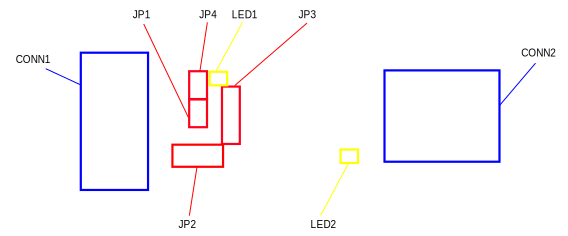
\includegraphics{images/usbprog_components}
  \caption{The USBprog device (version 3.0) with all connectors, jumpers and LEDs}
  \label{fig:usbprog}
\end{figure}


\subsection{Connectors}
\label{sec:connectors}

\begin{description}
  \item[\texttt{CONN1}] is the output interface which is used to do something useful with the
    USBprog beside from blinking LEDs. For example if you use the \emph{avrispmk2} firmware, this is
    an ISP interface which is used to program microcontrollers.

  \item[\texttt{CONN2}] is obviously the USB connector which is used to connect
    your USBprog to the computer. You have to use a \emph{Type B} cable which is the normal cable to
    connect USB devices---apart from micro or mini USB.
\end{description}


\subsection{Jumpers}
\label{sec:jumpers}

\begin{description}
  \item[\texttt{JP1}] (the lower two of the four pins) is the jumper that must be connected if
    the bootloader of the USBprog should be updated. See also section \vref{sec:inithardware} how to
    flash the bootloader.

  \item[\texttt{JP2}] controls how the power supply of the circuit that should be programmed
    (connected to \texttt{CONN1}). Figure \vref{fig:jp2} shows the possible connections:

    The default is no power supply for the programmed circuit. In that case you must ensure that the
    device is supplied with power by other means. This is the safest possibility.

    If you connect the two leftmost pins, that means that the 5~V VCC is directly from the USB port.
    This setting is dangerous because an error (short-circuit) in your circuit can damage the
    computer.

    An alternative is the setting of the two leftmost pins: In that case, the 5~V VCC is not
    directly from the USB port but with a Schottky diode. This is safer than the direct connection.

  \item[\texttt{JP3}] has two functions: At first it can be used as 5~V serial interface for
    debugging. You cannot directly connect this jumper to the computer but you need some level
    converter in between\footnote{If you want to build such a level converter yourself, look for
    example at \url{http://www.nslu2-linux.org/wiki/HowTo/AddASerialPort}. If you want to buy such a
    cable in Germany, the \href{http://www.eproo.net}{Embedded Project Shop} also has
    one. Look for ``FTDI-Kabel TTL-232R USB zu TTL serielles Kabel (5.0 V)''.}. This functionality
    is only needed by firmware developers.

    More important is another function which is used by the bootloader at startup. To put the device
    in update mode, disconnect the device, then connect pins 2 and 3 as shown in figure
    \vref{fig:jp3} and connect the device again.

  \item[\texttt{JP4}] is application specific, i.\,e. used directly by the firmware that is flashed
    into the USBprog. Currently, \texttt{JP4} is not used by any of the public firmwares.
\end{description}

\begin{figure}[thb]
  \centering
  
\includegraphics{images/jp2}
  \caption{Possible connections of \texttt{JP2}}
  \label{fig:jp2}
\end{figure}

\begin{figure}[thb]
  \centering
  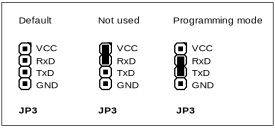
\includegraphics{images/jp3}
  \caption{Possible connections of \texttt{JP3}}
  \label{fig:jp3}
\end{figure}


\subsection{LEDs}
\label{sec:leds}

\begin{description}
  \item[\texttt{LED1} (red)] is used by the firmware. There are two common scenarios:

    If the USBprog is in \emph{update mode,} the LED blinks slowly. In the wide-spread Atmel MTK II
    clone firmware, this LED shines while the programming of the microcontroller is ongoing.

  \item[\texttt{LED2} (green)] is just the Power LED.
\end{description}


\section{Initialise the Hardware}
\label{sec:inithardware}

This section describes how to install the bootloader. If you bought a version of USBprog which
already contains the bootloader, you can safely skip that step. If you don't know if you have a
version with bootloader, please read section \vref{sec:check_if_bootloader_installed}.


\subsection{Check if the Bootloader is Installed}
\label{sec:check_if_bootloader_installed}

% TODO


\subsection{Flashing the Bootloader}

When buying a USBprog at the \href{http://www.eproo.net}{Embedded Projects Webshop} you can choose
between a slightly cheaper version without an already flashed bootloader and a slightly more
expensive version that already has flashed the bootloader.

Flashing the bootloader is the only step where you need a second programming device. It's possible
to use an already initialised USBprog with the ``AVRISP mk2 Clone'' firmware flashed. Any other
programmer for Atmel AVR microcontrollers will do it, too. You need the standardised \emph{ISP}
interface.

In the rest of the document we assume that you have already a USBprog and you want to initialised a
second one. It should be easy to use that description for another programmer since the
\emph{AVRdude} software supports basically every AVR programmer that is out there.








% \bibliography{literatur}
\bibliographystyle{IEEEtran}

% \begin{thebibliography}{999999}
%   \bibitem[bla]{fasel} df
% \end{thebibliography}


\end{document}

% vim: set sw=2 ts=2 et spell spelllang=en_gb tw=100:
